\begin{figure}
\centering
\resizebox{\columnwidth}{!}{
\begin{tabular}{@{} c c @{}}
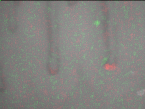
\includegraphics[width=0.5\columnwidth]{\figpath/real_flow/u_overlay} &
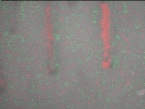
\includegraphics[width=0.5\columnwidth]{\figpath/real_flow/v_overlay} \\
(a) & (b)
\end{tabular}}
%
\caption{Real image (\fref{fig_example_images}) overlaid with estimated image flow in the (a) horizontal and (b) vertical directions. Because flow magnitude is not available for this real sequence, the colouring instead indicates the direction of flow over the sequence: green is right/down; red is left/up. The intensity denotes the proportion of the sequence in the given direction. The regions of flow in the two vessels are clear.}
\label{fig_flow_results}
\end{figure}
